\documentclass[11pt,french,a4paper]{article}

\usepackage{enumitem}
\usepackage{graphicx}
\usepackage{listings}
\usepackage{multicol}
\usepackage{titling}
\usepackage{hyphenat}

\usepackage[francais,box,completemulti]{automultiplechoice}
\usepackage{hyperref}
\title{Projet d'intégration de développement}
\date{\today}
\author{François ROLAND}
\AMCrandomseed{1}
\hypersetup{
  pdftitle={\thetitle},
  pdfauthor={\theauthor},
  pdflang={fr-BE},
  hidelinks}
\usepackage{polyglossia}
\setdefaultlanguage{french}
\usepackage{csquotes}
\geometry{hmargin=2cm,headheight=2cm,headsep=.3cm,footskip=1cm,top=3cm,bottom=2cm}
\begin{document}

%%% preparation of the groups

% chktex-file 19
\setdefaultgroupmode{withoutreplacement}

\element{q001}{
  \begin{questionmult}{objectifs}
    Quels sont les objectifs principaux d'un cahier des charges~?
    \begin{choices}
      \correctchoice{Communiquer le but du projet.}
      \correctchoice{Planifier les moyens à allouer.}
      \correctchoice{Vérifier que le projet est toujours pertinent et que les objectifs sont atteints.}
      \wrongchoice{Dessiner des diagrammes.}
      \wrongchoice{Raccourcir les délais d'analyse.}
      \wrongchoice{S'assurer que le projet ne sera jamais arrêté de manière précoce.}
      \wrongchoice{Éliminer toutes les inconnues du projet.}
    \end{choices}
  \end{questionmult}
}

\element{q002}{
  \begin{question}{diag-contexte}
    Que représente un diagramme UML de contexte~?
    \begin{choices}
      \correctchoice{Les acteurs et la manière dont ils interagissent avec le système.}
      \wrongchoice{Les parties prenantes et la manière dont elles interagissent avec le système.}
      \wrongchoice{Les acteurs et la manière dont ils interagissent dans le projet.}
      \wrongchoice{Les parties prenantes et la manière dont elles interagissent dans le projet.}
    \end{choices}
  \end{question}
}

\element{q003}{
  \begin{question}{acteur-primaire}
    Qu'est-ce qu'un acteur primaire~?
    \begin{choices}
      \correctchoice{Une personne ou un système qui est à l'origine des interactions avec le système.}
      \wrongchoice{Une personne ou un système important.}
      \wrongchoice{Une personne ou un système qui n'est pas directement à l'origine des interactions avec le système.}
      \wrongchoice{Une personne ou un système dont les cas d'utilisation sont traités en priorité.}
    \end{choices}
  \end{question}
}

\element{q003}{
  \begin{question}{acteur-secondaire}
    Qu'est-ce qu'un acteur secondaire~?
    \begin{choices}
      \correctchoice{Une personne ou un système qui n'est pas directement à l'origine des interactions avec le système.}
      \wrongchoice{Une personne ou un système qui est à l'origine des interactions avec le système.}
      \wrongchoice{Une personne ou un système important.}
      \wrongchoice{Une personne ou un système dont les cas d'utilisation sont traités en priorité.}
    \end{choices}
  \end{question}
}

\element{q004}{
  \begin{question}{besoin-fonctionnel}
    \enquote{En tant que bibliothécaire, je veux rechercher un livre sur base du titre et de l'auteur afin de retrouver l'emplacement où il est rangé.}

    De quel type de besoin s'agit-il~?
    \begin{multicols}{3}\AMCBoxedAnswers{}
      \begin{choices}
        \correctchoice{Besoin fonctionnel.}
        \wrongchoice{Besoin non fonctionnel.}
        \wrongchoice{Contrainte.}
        \wrongchoice{Besoin primaire.}
        \wrongchoice{Besoin secondaire.}
      \end{choices}
    \end{multicols}
  \end{question}
}

\element{q005}{
  \begin{question}{singletable}
    Observez le diagramme suivant.

    \begin{center}
      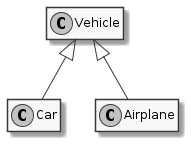
\includegraphics[width=4cm]{class_inheritance.png}
    \end{center}

    En vous basant uniquement sur ces diagrammes, déterminer à quelle(s) classe(s) appartient l'attribut \texttt{altitudeMax}.
    \begin{multicols}{2}\AMCBoxedAnswers{}
      \begin{choices}
        \correctchoice{Les informations fournies ne sont pas suffisantes pour déterminer la classe.}
        \wrongchoice{\texttt{Vehicle}.}
        \wrongchoice{\texttt{Car}.}
        \wrongchoice{\texttt{Airplane}.}
        \wrongchoice{\texttt{Car} et \texttt{Airplane}.}
      \end{choices}
    \end{multicols}
  \end{question}
}


%%% copies

\onecopy{16}{
  \setlength{\parindent}{0pt}
  %%% beginning of the header
  \noindent{{\LARGE{\nohyphens{\thetitle}}}}

  \vspace{2em}

  \noindent{\setlength{\parindent}{0pt}\hspace*{\fill}\AMCcodeGridInt{etu}{5}\hspace*{\fill}
  \begin{minipage}[b]{.6\linewidth}
    $\longleftarrow{}$\hspace{0pt plus 1cm} Codez votre matricule d'étudiant ci-contre et écrivez la date ainsi que vos nom et prénom tels qu'ils apparaissent sur le document d'identité présenté lors de votre inscription à l'intérieur des cadres ci-dessous.

    \vspace{1.5em}

    \fbox{\begin{minipage}[b]{\linewidth}%
      {\footnotesize Date \par}%
      \vspace{5mm}\dotfill%
      \vspace*{1mm}%
      \end{minipage}}

    \vspace{.5em}

    \namefield{\fbox{\begin{minipage}[b]{\linewidth}%
      {\footnotesize Nom et prénom \par}%
      \vspace{5mm}\namefielddots{}%
      \vspace*{1mm}%
      \end{minipage}}}
  \end{minipage}}

  \noindent\hrulefill{}
  \begin{itemize}[nosep]
    \item Répondez aux questions à l'aide d'une croix dans la case correspondant à votre réponse.
    \item Les questions avec le symbole \multiSymbole{} peuvent avoir zéro, une ou plusieurs bonnes réponses.
          Les autres ont une seule bonne réponse.
    \item Vous pouvez \enquote{décocher} une case en la noircissant, sans laisser d'espace blanc.
    \item Rien de ce qui est écrit ou dessiné en dehors des cases à cocher ne sera pris en compte.
    \item Afin de faciliter la lecture optique, utilisez un bic bleu ou noir.
  \end{itemize}
  \noindent\hrulefill{}
  \vspace*{1.5em}

  %%% end of the header

  \cleargroup{all}

  \copygroup[1]{q001}{all}
  \copygroup[1]{q002}{all}
  \copygroup[1]{q003}{all}
  \copygroup[1]{q004}{all}
  \copygroup[1]{q005}{all}

  \insertgroup{all}

  \AMCcleardoublepage{}
}


\end{document}
